\documentclass{article}
\usepackage{pgfplots}
\pgfplotsset{compat=1.18}
\usepackage{amsmath}

\begin{document}

\begin{figure}[h]
    \centering
    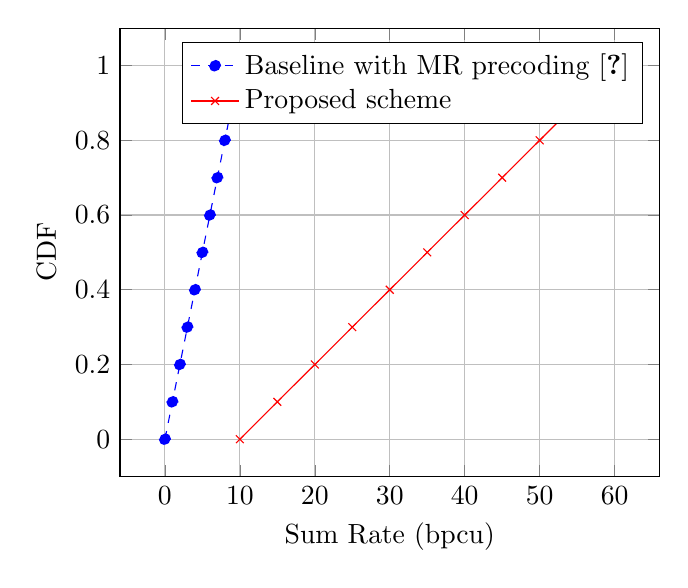
\begin{tikzpicture}
        \begin{axis}[
            xlabel={Sum Rate (bpcu)},
            ylabel={CDF},
            grid=major,
            legend pos=north east,
            legend cell align={left},
            clip=false % Add this line to ensure the legend fully appears
        ]
            \addplot[blue, dashed,mark=*] coordinates {
                (0,0) (1,0.1) (2,0.2) (3,0.3) (4,0.4) (5,0.5) (6,0.6) (7,0.7) (8,0.8) (9,0.9) (10,1)
            };
            \addlegendentry{Baseline with MR precoding \cite{antonioli2023mixed}};
            
            \addplot[red, mark=x] coordinates {
                (10,0) (15,0.1) (20,0.2) (25,0.3) (30,0.4) (35,0.5) (40,0.6) (45,0.7) (50,0.8) (55,0.9) (60,1)
            };
            \addlegendentry{Proposed scheme};
        \end{axis}
    \end{tikzpicture}
    \caption{Performance comparison between Baseline with MR precoding~\cite{antonioli2023mixed} and Proposed scheme. Parameters: $L=10$, $M=5$, $K=5$, and $N=1$.}
    \label{fig:performance_comparison}
\end{figure}

\end{document}